\documentclass[11pt]{article}
\usepackage[margin=1in]{geometry}
\usepackage{fontspec}
\setmainfont{Times New Roman}
\setsansfont{Arial}
\setmonofont{Menlo}
\usepackage{amsmath,amssymb,graphicx,booktabs}
\usepackage[unicode,hidelinks]{hyperref}
\usepackage{xurl}
\urlstyle{same}
\setlength{\emergencystretch}{5em}
\setlength{\parindent}{0pt}
\setlength{\parskip}{6pt plus 2pt}
\setcounter{secnumdepth}{-1}
\providecommand{\tightlist}{\setlength{\itemsep}{0pt}\setlength{\parskip}{0pt}}
\newcommand{\pandocbounded}[1]{#1}
\pagestyle{plain}
\begin{document}
\section{Passing Coarse Marginal Checks Can Be Cheap: Persona Mixtures
and Imprecise Treatment-Response Estimates in an LLM Persona
Panel}\label{passing-coarse-marginal-checks-can-be-cheap-persona-mixtures-and-imprecise-treatment-response-estimates-in-an-llm-persona-panel}

Yohei Nakajima\\
Untapped Capital

\subsection{Abstract}\label{abstract}

Large language models are used as synthetic participants, often
validated through resemblance to human marginal responses. A fixed panel
of sixteen persona-conditioned GPT-4.1 prompts met preregistered
broad-reference mean criteria in three of four repeated-game cells.
Between-prompt variation was substantial but prior-sensitive. Aggregate
continuation-probability contrasts were +0.083 and +0.078, with
model-based simultaneous intervals {[}−0.171, +0.330{]} and {[}−0.181,
+0.330{]}. The treatment changed both continuation and its textual
representation. Separate representation operations produced large choice
shifts without identifying a unique mechanism. External review exposed
dependence and multiplicity defects; additive reanalysis preserved the
historical record while withdrawing a favored persona-level
interpretation. These findings show what coarse validation left
imprecisely estimated in one fixed deployment. They establish neither a
zero response nor equivalence, human treatment-effect error, or human
substitutability. The released archive supports credential-free replay.

\subsection{1. Introduction}\label{introduction}

A synthetic participant may produce plausible aggregate choices without
supplying precise evidence about the response object an experiment
needs. Here, ``cheap'' denotes evidentiary economy: a validation
criterion can be satisfied without requiring that evidence. We examine
one fixed sixteen-prompt panel in strategic interaction. Three of four
repeated-game condition means passed broad preregistered reference
bands, while continuation-probability response estimates remained
imprecise.

This question belongs to experimental validation rather than a general
verdict on artificial intelligence. Algorithmic fidelity (Argyle et al.,
2023), simulated economic agents (Horton, 2023), and behavioral
similarity tests (Mei et al., 2024) provide reasons to investigate
synthetic participants. Li and Ji (2026) show that statistical realism
can diverge from treatment-effect accuracy; Persson et al.~(2026) state
causal-surrogacy assumptions; Lin et al.~(2026) diagnose latent-user
drift under intervention. We do not claim to discover that divergence or
exhaust its mechanisms.

The closest JESA comparison is Polachek et al.~(2025), who compare LLM
prisoner's-dilemma choices with a human experiment while varying stakes,
order, and framing. Prompt sensitivity and imperfect imitation are
already established territory. Our narrower addition is a registered,
fixed-panel decomposition of between-prompt composition, within-prompt
variation, and represented continuation response, coupled with an
explicit dependence and correction record. Unlike their human
comparison, our protocol-nonmatched human references cannot identify
human treatment-effect error.

Repeated-game prompting and parameter variation also precede this study
(Akata et al., 2025; Pal et al., 2026). Strong effect forecasting across
human studies is positive evidence for a different use: Ashokkumar et
al.~(2026) forecast experimental effects, rather than construct the
subject-level response surface examined here. Calibration (Hullman et
al., 2026) and latent-drift diagnostics can complement our fixed-panel
analysis. The later respondent-coverage study of Kumagae and Kaneko
(2026), posted after our August preprint, likewise distinguishes answer
marginals from joint respondent profiles; its survey coverage target
differs from our strategic-response target. Supplement S1 retains the
broader literature and exact versions.

\subsection{2. Design and estimands}\label{design-and-estimands}

The primary historical deployment used GPT-4.1, temperature 0.7, and
outputs capped at sixteen tokens. A minimal subject prompt supplied no
reasoning scaffold or game-theory vocabulary. The OpenAI-compatible
adapter supplied temperature and \texttt{max\_tokens=16};
\texttt{top\_p=1} was specified in the assembly but omitted from the
wire. Other sampling penalties inherited provider defaults. No tools or
native structured output were used. Environment randomness was seeded;
provider generation was not claimed to be seeded.

Before Phase 5 dispatch, a seeded registry generated sixteen complete
persona sentences from two age bands and three binary trait dimensions:
agreeable/competitive, patient/impulsive, and risk-averse/risk-seeking.
Cooperative leaning meant at least two of agreeable, patient, and
risk-averse, yielding eight prompts per stratum without reference to
behavior. Names and occupations are uncontrolled semantic components.
Each complete sentence was prepended to sealed task text. The panel is a
fixed construction, not a probability sample of people or a persona
generator.

Phase 5 crossed these prompts with four repeated prisoner's-dilemma
cells (continuation probabilities .10/.90 × wording families S2
absent/present), a one-shot label swap, and a Community frame. Primary
repeated cells have six complete episodes each. Two seats share an
episode; calls, rounds, and seats are not independent subjects. For
prompt \(i\), condition \(d\), and episode \(e\), the round-one
cooperation outcome is \(Y_{ide}\in\{0,0.5,1\}\), the fraction of its
two seats cooperating. Define \(p_i(d)=E[Y_{ide}\mid i,d]\) and the
equally weighted fixed-panel mean \(\bar p(d)=16^{-1}\sum_i p_i(d)\).
The aggregate represented-treatment contrast is
\(\Delta=\bar p(.90)-\bar p(.10)\) within each wording family.

The continuation intervention changed the stochastic environment and the
sentence communicating it jointly. It identifies response to that
represented treatment, not an isolated incentive effect. Reusing
explicit prompt text identifies a prompt-indexed contrast; it does not
establish a stable latent person's potential outcomes. The deployment,
prompt, condition, episode, seat, round, and request levels must remain
distinct.

Phase 3 tested the bare instrument; Phase 4 studied representation,
labels/payoffs, continuation, adversaries, and monitoring; Phase 5 added
the persona panel. Phase 1--2 development is exploratory. Confirmatory
predicates preceded their adjudicating data, including sequential X1
registration after Phase 3. Some later design choices were
result-informed prospective amendments, and the present sensitivity
analyses are post-adjudication. Supplement S2 links the actual seals,
dispatch, amendments, adjudications, and reviewer role changes;
draft-looking sealed headers are preserved rather than rewritten.

\subsubsection{2.1 Uncertainty and validation
criteria}\label{uncertainty-and-validation-criteria}

We use the episode, retaining uncertainty when observed cells are
unanimous. Write \(A=\mathbf 1(Y\ge0.5)\) and \(B=\mathbf 1(Y=1)\), so
\(Y=(A+B)/2\). Simultaneous Clopper--Pearson component intervals project
onto condition means. Four component-condition intervals split the error
rate by Bonferroni for each contrast. If the projected intervals are
\([L_d,U_d]\), the reported contrast interval is
\([L_{.90}-U_{.10},U_{.90}-L_{.10}]\). This conservative discrete
small-sample construction uses independent episodes and a pooled
component-binomial working model; prompt heterogeneity and the precise
coverage domain require care (Supplement S3). It is distinct from
treating two seats as independent Bernoulli trials (Clopper and Pearson,
1934).

Three composition views are intentionally separated.
Finite-opportunity-corrected plug-in estimates and conditional episode
bootstraps describe the recorded panel; unanimous cells remain
degenerate in that bootstrap. Symmetric Dirichlet priors on each
prompt-cell's three outcome probabilities propagate sparse-cell
uncertainty but are prior-sensitive. A two-stage prompt-plus-episode
bootstrap changes the target toward a hypothetical persona generator.
These are different conditioning assumptions, not independent
replications of one estimate.

Table 1 distinguishes the validation criterion from the desired
inference. Broad condition-specific bands \([\ell_d,u_d]\) imply only
\(\Delta\in[\ell_1-u_0,u_1-\ell_0]\). Exact matching of both means would
fix their difference; our point concerns slack in coarse criteria. The
law of total variance and classical coupling results explain why
marginal moments do not determine between/within composition or
cross-condition coupling (Supplement S3); these applications are not new
probability theorems.

\begin{tabular}{p{.17\linewidth}p{.37\linewidth}p{.35\linewidth}}\toprule
Target & Criterion or estimate & What it supports \\ \midrule
Marginal level & Reference band [.36,.63]; 3/4 means inside & Passage of a broad historical check \\
Composition & Plug-in 85–96\%; Dirichlet medians depend on prior & Substantial prompt-indexed variation in this panel \\
Aggregate response & +.083 / +.078; simultaneous intervals about −.18 to +.33 & Imprecise represented-treatment response \\
Latent-person response & No invariance test & Unidentified \\
Human causal accuracy & Protocol-nonmatched references & Unidentified \\
\bottomrule\end{tabular}

Table 1. Validation targets, evidence, and inference limits. Composition
percentages are between-prompt shares of episode-level variation.
Neither the bands nor the variance heuristic is an equivalence margin.

\subsection{3. Results}\label{results}

\subsubsection{3.1 Marginal fit and
composition}\label{marginal-fit-and-composition}

Repeated-cell cooperation means were 0.349, 0.427, 0.432, and 0.505; the
sole reference-band miss was 0.011 below the lower bound.
Cooperative-leaning minus defect-leaning prompt-bundle differences were
0.510--0.719. They are not isolated causal trait effects.

Between-prompt plug-in shares were 85.5\%, 96.1\%, 88.8\%, and 90.2\%.
Fixed-panel Jeffreys Dirichlet(\(0.5,0.5,0.5\)) posterior medians were
63.1\%, 70.5\%, 66.1\%, and 66.6\%; respective 95\% intervals were
{[}49.4\%,74.5\%{]}, {[}57.3\%,81.3\%{]}, {[}52.7\%,77.1\%{]}, and
{[}52.7\%,77.7\%{]}. A symmetric-prior sweep yielded medians
74.8--82.5\% at \(\alpha=.25\) and 47.1--53.5\% at \(\alpha=1\). Thus
substantial composition persists, but a share exceeding one-half is
prior-dependent (Figure 1).

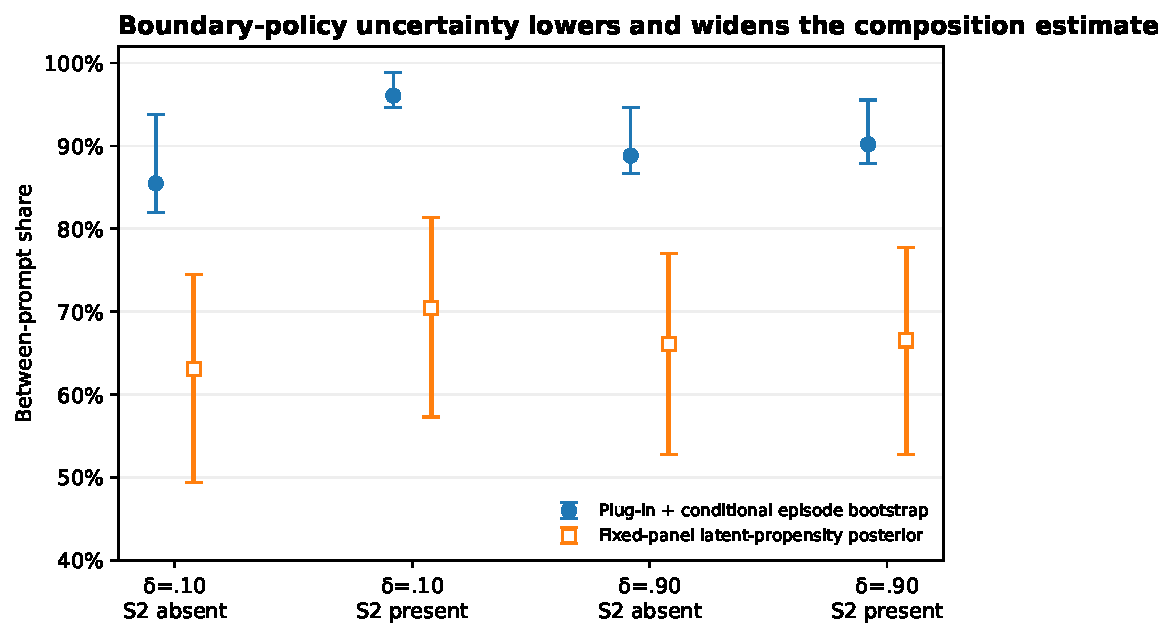
\includegraphics[width=.95\linewidth]{figures/between-prompt-share.pdf}

Figure 1. Plug-in/conditional-bootstrap and Jeffreys fixed-panel
composition estimates. The former conditions on recorded corner
concentration; the latter shrinks sparse cells inward. Uniform-prior
medians reported in text straddle one-half. These estimates are not
interchangeable.

P5-1b compared corrected dispersion with heuristic thresholds derived
from Dal Bó and Fréchette's (2011) human strategy frequencies. Those
experiments differ in continuation, payoffs, incentives, assignment, and
experience. The frozen ratio .75 is a tolerance, not a human-equivalence
margin. The historical dispersion checkpoint is permissive; neither its
passage nor matched-looking SD establishes human variance equivalence.

The binary interiority census is also method-sensitive. In the
registered restricted set, the frozen seat rule classified 3/32 cells
interior, the episode-exact rule 2/32, and Jeffreys sensitivity 5/32.
Across all six conditions, the corresponding counts are 14/96, 11/96,
and 19/96. Six episodes and discrete outcomes make threshold labels
unstable; continuous estimates are more informative.

\subsubsection{3.2 Response and
representation}\label{response-and-representation}

Continuation contrasts were +0.083 (S2 absent) and +0.078 (S2 present).
Under the pooled component-binomial working model, simultaneous 95\%
intervals were {[}−0.171,+0.330{]} and {[}−0.181,+0.330{]}. These are
exact descriptive differences for the archived panel but imprecise
estimates of its repeated-sampling propensities. They establish neither
equivalence, zero response, nor a narrow upper bound (Figure 2). A
coarse validation design did not require this response object to be
precisely estimated.

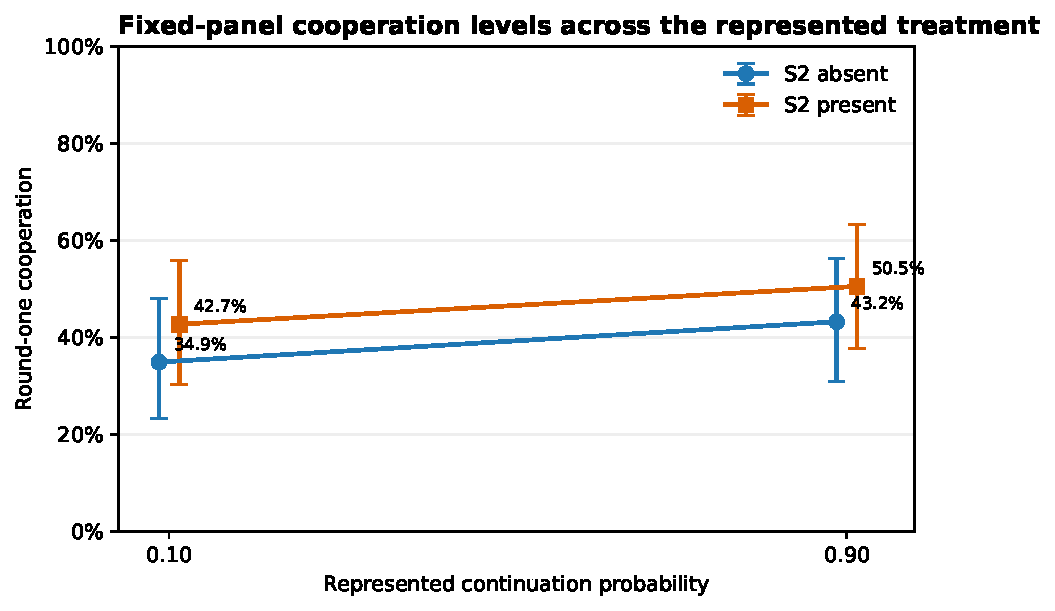
\includegraphics[width=.95\linewidth]{figures/condition-means.pdf}

Figure 2. Cooperation levels and episode-based condition intervals under
the pooled component-binomial working model. Lines orient the eye;
contrast intervals in text use simultaneous component projection.
Process and communicating text change together.

For the bare configuration, a screened and held-out S2
wording-and-position replacement shifted cooperation from 0/40 to 37/40
seat choices. Wording and position were one operation. By contrast,
ordinary one-shot wording had a registered main effect of +0.0063 (SE
.0210; Holm-adjusted \(p=1.00\)). Announcing and implementing repeated
interaction produced larger changes, including ceiling-confounded cells;
those ceilings cannot identify a continuation slope.

With canonical payoffs held fixed, swapping ``Cooperate'' and ``Defect''
made the bare configuration always choose the dominated role labeled
``Defect.'' This demonstrates label-linked control in that cell, but
learned game associations and intrinsic lexical valence are not
separated. Adding a persona reversed the bare choice; no format-matched
neutral prefix was tested, and label and payoff then favored the same
option. Neither operation isolates a universal semantic mechanism.

P5-2 pooled 90/704 seat decisions across 352 episodes, equivalently an
episode mean of 45/352=.128. The principal dependence-aware sensitivity,
a stratified bootstrap over forty prompt-by-conflict clusters, gave
{[}.071,.189{]}. Fixed-panel Dirichlet aggregation moved from median
.138 at \(\alpha=.10\) to .205 at \(\alpha=1\), whose interval
{[}.182,.231{]} crosses the registered .20 boundary. The historical
verdict remains visible; Bayesian proximity to its boundary is not
prior-robust corroboration. Repeated conflict subcells were mixed; the
pooled dominance classification is carried by the word/payoff-confounded
swap cell.

\subsubsection{3.3 Multiplicity and the withdrawn persona
interpretation}\label{multiplicity-and-the-withdrawn-persona-interpretation}

The frozen P5-3(a) search selected persona p13 after searching multiple
persona-by-wording candidates without prospective family control. Its
apparent capability finding is withdrawn. Three post-adjudication
200,000-permutation analyses dynamically reapply their eligibility gates
in every draw. Add-one familywise \(p\) values and Monte Carlo 95\%
intervals are .059230 {[}.058194,.060268{]} under the historical seat
gate; .043455 {[}.042561,.044353{]} under the percentile
episode-bootstrap gate; and .773206 {[}.771363,.775039{]} for the
largest eligible candidate p05 under the conservative exact gate, where
p13 is ineligible.

The favorable bootstrap variant cannot create prospective confirmation;
none was sealed before computation. Conversely, the exact gate cannot
decisively disconfirm the capability. At six episodes, its eligible
compositions permit a maximum slope .333; the archived family's
estimated minimum attainable familywise tail probability is .075040
{[}.073884,.076198{]}, above .05. P13 is a prospective replication
target, not an established finding or a decisive negative. No new study
is needed for the present bounded conclusion.

No study-wide alpha allocation was registered across P5 predicates and
X1. Registered block-specific controls, including Holm-controlled
adversary tests, retain their own scope. The complete supplementary
record retains favorable and unfavorable variants, dead predictions,
invalidations, and secondary findings. Mechanical predicate enforcement
cannot ensure construct validity or an appropriate family.

\subsection{4. Implications and
limitations}\label{implications-and-limitations}

Validation should name the target, intervention representation,
dependence unit, and uncertainty required for the intended use. A panel
can pass a coarse level check while leaving treatment response loosely
bounded. This is a limitation of the criterion demonstrated in one fixed
deployment, not evidence that matched human responses would be
different.

The model version and sixteen bundled prompts bound generalization.
Prompt pairing does not establish latent-person invariance; no new human
comparison, wider persona sample, factorial mechanism control, or
endpoint refresh is claimed. Gemini observations are descriptive because
its unversioned endpoint drifted. Temperature interactions outside the
frozen plan are exploratory. More episodes may improve within-prompt
precision, but a wider persona-generator claim requires a declared
sampling design.

Auditability enabled correction rather than self-validation. A sealed
pre-data discussion originally interpreted p13 as an incentive-response
existence result; review exposed dependence, family-error, and construct
defects. The original discussion, mechanical verdicts, seals, and
amendment history remain unchanged. One AI reviewer later helped specify
post-adjudication analyses; this role transition and later independent
checks are disclosed in Supplement S2. The human author retains
responsibility. These records preserve the distinction between
registered predictions, result-informed prospective changes, descriptive
observations, and later reinterpretation.

\subsection{5. Data, code, and
declarations}\label{data-code-and-declarations}

The immutable evidence baseline is repository commit
\nolinkurl{62ab90beff1d291b069c87f13b6b6b3495171ddd}; the distinct
public preprint is arXiv:2608.00979v1. Supplement S4 and the separate
Data and Instructions appendix link the code, registrations, complete
prompts, data dictionary, licenses, and audit receipts. The archive
contains 4,916 confirmatory runs: 320 Phase 3/X1 LLM, twenty
deterministic baselines, 2,864 Phase 4, and 1,712 Phase 5. Three legacy
diagnostics raise the verifier boundary to 4,919 runs, of which 4,899
are LLM runs; runs are not provider calls.

Phase 3 lacks the richer response IDs and request-body hashes of Phases
4--5. The latter contain 30,421 request events and 30,397 response
events; twenty-four failed-run partials are excluded from completed
analyses but retained in accounting. Snapshot checksums and timestamps
detect changes relative to publication; they are not provider
attestation or proof of immutability from receipt. Replay reconstructs
archived behavior without live models and cannot establish human
validity or adequate power.

Author affiliation/contact/ORCID, contributions, actual funding/support,
interests, human-data determination, rights, full AI assistance history,
and current journal history await author confirmation in a separate
worksheet. This review candidate must not be submitted with unresolved
declarations. Subject-model apparatus and AI assistance are distinct:
archived subject models generated observations; AI coding, writing,
analysis, and adversarial-review roles require the author-approved
disclosure. AI systems are not authors.

\begingroup\small\setlength{\parskip}{3pt}\subsection{References}\label{references}

Akata, E., Schulz, L., Coda-Forno, J., Oh, S. J., Bethge, M., and
Schulz, E. (2025). Playing repeated games with large language models.
\emph{Nature Human Behaviour, 9}, 1380--1390.
\url{https://doi.org/10.1038/s41562-025-02172-y}

Argyle, L. P., Busby, E. C., Fulda, N., Gubler, J. R., Rytting, C., and
Wingate, D. (2023). Out of one, many: Using language models to simulate
human samples. \emph{Political Analysis, 31}(3), 337--351.
\url{https://doi.org/10.1017/pan.2023.2}

Ashokkumar, A., Hewitt, L., Ghezae, I., and Willer, R. (2026). Large
language models can predict the results of social science experiments.
\emph{Nature, 656}, 115--122.
\url{https://doi.org/10.1038/s41586-026-10742-x}

Clopper, C. J., and Pearson, E. S. (1934). The use of confidence or
fiducial limits illustrated in the case of the binomial.
\emph{Biometrika, 26}(4), 404--413.
\url{https://doi.org/10.1093/biomet/26.4.404}

Dal Bó, P., and Fréchette, G. R. (2011). The evolution of cooperation in
infinitely repeated games: Experimental evidence. \emph{American
Economic Review, 101}(1), 411--429.
\url{https://doi.org/10.1257/aer.101.1.411}

Horton, J. J. (2023). Large language models as simulated economic
agents: What can we learn from Homo Silicus? NBER Working Paper 31122,
original April 2023 version.
\url{https://www.nber.org/system/files/working_papers/w31122/revisions/w31122.rev0.pdf}.
\url{https://doi.org/10.3386/w31122}

Hullman, J., Broska, D., Sun, H., and Shaw, A. (2026). This human study
did not involve human subjects: Validating LLM simulations as behavioral
evidence. arXiv:2602.15785v1. \url{https://arxiv.org/abs/2602.15785v1}.
\url{https://doi.org/10.48550/arXiv.2602.15785}

Kumagae, Y., and Kaneko, M. (2026). Silicon samples match the answers
but not the respondents. arXiv:2610.30900v1.
\url{https://arxiv.org/abs/2610.30900v1}.
\url{https://doi.org/10.48550/arXiv.2610.30900}

Li, Z., and Ji, F. (2026). Statistical realism is not evidence that LLMs
can estimate treatment effects in social science experiments.
arXiv:2604.02458v3. \url{https://arxiv.org/abs/2604.02458v3}.
\url{https://doi.org/10.48550/arXiv.2604.02458}

Lin, V., Yun, T., Matarić, M. J., Canny, J., Gretton, A., and D'Amour,
A. (2026). The illusion of intervention: Your LLM-simulated experiment
is an observational study. arXiv:2605.20767v1.
\url{https://arxiv.org/abs/2605.20767v1}.
\url{https://doi.org/10.48550/arXiv.2605.20767}

Mei, Q., Xie, Y., Yuan, W., and Jackson, M. O. (2024). A Turing test of
whether AI chatbots are behaviorally similar to humans.
\emph{Proceedings of the National Academy of Sciences, 121}(9),
e2313925121. \url{https://doi.org/10.1073/pnas.2313925121}

Pal, S., Mallela, A., Hilbe, C., Pracher, L., Wei, C., Fu, F., Schnell,
S., and Nowak, M. A. (2026). Strategies of cooperation and defection in
five large language models. arXiv:2601.09849v1.
\url{https://arxiv.org/abs/2601.09849v1}.
\url{https://doi.org/10.48550/arXiv.2601.09849}

Persson, J., Schultzberg, M., and Ankargren, S. (2026). Statistical
foundations of LLM-based A/B testing: A surrogacy framework for human
causal inference. arXiv:2606.17165v3.
\url{https://arxiv.org/abs/2606.17165v3}.
\url{https://doi.org/10.48550/arXiv.2606.17165}

Polachek, S. W., Romano, K., and Tonguc, O. (2025). Homo-silicus: not
(yet) a good imitator of homo sapiens or homo economicus. \emph{Journal
of the Economic Science Association, 11}(2), 261--269.
\url{https://doi.org/10.1017/esa.2025.10023}
\endgroup
\end{document}
